\documentclass[a4paper,10pt]{article}
\usepackage[utf8]{inputenc}
\usepackage{polski}
\usepackage{graphicx}
\usepackage{listings}
\usepackage[usenames,dvipsnames]{color}
\addtolength{\hoffset}{-1cm}
\addtolength{\voffset}{-2cm}
\addtolength{\textwidth}{2cm}
\addtolength{\textheight}{3cm}
\usepackage{setspace}
\usepackage{indentfirst}
\usepackage{graphicx}
\lstset{
    language=Matlab,
    basicstyle=\scriptsize,
    aboveskip={1.5\baselineskip},
    columns=fixed,
    showstringspaces=false,
    extendedchars=true,
    breaklines=true,
    tabsize=4,
    prebreak = \raisebox{0ex}[0ex][0ex]{\ensuremath{\hookleftarrow}},
    frame=single,
    showtabs=false,
    showspaces=false,
    showstringspaces=false,
    identifierstyle=\ttfamily,
    keywordstyle=\color[rgb]{0,0,1},
    commentstyle=\color[rgb]{0.133,0.545,0.133},
    stringstyle=\color[rgb]{0.627,0.126,0.941},
    numbers=left,
    numberstyle=\tiny,
    stepnumber=1,
    numbersep=5pt,
    captionpos=b,
    escapeinside={\%*}{*)}
}

\def\figurename{Rys.}
\def\lstlistingname{Fun.}

\title{Informatyczne Systemy Sterowania \\ \large Ćwiczenie 4: Sterowanie ekstremalne}

\author{Adam Jordanek 168139, Tomasz Klimek 168092}

\begin{document}
\maketitle

\section{Wstęp}\label{sec:wstęp}
\subsection{Cel ćwiczenia}
%TODO!!!!! SKOPIOWANE Z LISTY
Celem  ćwiczenia jest symulacja działania systemu sterowania ekstremalnego. Sterowaniem 
ekstremalnym nazywamy zadanie sterowania polegające na doprowadzeniu poprzez odpowiednią
zmianę wielkości sterujących do ekstremalnej wartości wielkości sterowanej (lub ekstremalnych 
wartości wielkości sterowanych w przypadku obiektu wielowyjściowego)

\subsection{Plan badań} 
\begin{enumerate}
	\item Symulacja systemu sterowania ekstremalnego - Algorytm 1
	
	\item Symulacja systemu sterowania ekstremalnego - Algorytm 2
	
	\item Symulacja systemu sterowania ekstremalnego - Algorytm 3
	
\end{enumerate}

\subsection{Podział zadań. } 
\begin{enumerate}
		\item Jordanek Adam - 
		\item Klimek Tomasz -
\end{enumerate}

\newpage
\section{Realizacja planu i wyniki}
W zadaniu sterować będziemy dwa obiekty przedstawione przy pomocy poniższych równań.
\begin{eqnarray}
	y = F(u, a, b, c) = (u^{(1)} - a)^2 + (u^{(2)} - b)^2 + c\\
	y = F(u, a, b, c, A, B, \omega_1, \omega_2, t) = (u^{(1)} - (a + Asin(\omega_1t)))^2 + (u^{(2)} - (b + Bsin(\omega_2t)))^2 + c
\end{eqnarray}
Podczas ćwiczenia przyjęliśmy następujące wartości parametrów. \\
$a=1, b=2, c=3, A=2, B=4, \omega_1=0.5, \omega_2=0.25$
%--------------------------------------------------------------------------------------------------------------------------------
%ZADANIE 1
%--------------------------------------------------------------------------------------------------------------------------------
\subsection{Symulacja systemu sterowania ekstremalnego – wersja 1. algorytmu.}

\subsubsection{Obiekt (1).}
W pierwszym zadaniu do wyznaczenia ekstremów posłuży nam poniższa funkcja.
\begin{eqnarray}
	u_n^{(i)} = u_{n-1}^{(i)}-kd_n^{(i)}\\
	d_n^{(i)} = {F(u_{n-1}) - F(u_{n-2}) \over u_{n-1}^{(i)} - u_{n-2}^{(i)}}
\end{eqnarray}

Jednak dla ułatwienia ćwiczenia powyższy algorytm zmodyfikujemy do poniższej postaci.
\begin{eqnarray}
	u_n^{(i)} = u_{n-1}^{(i)}-kd_n\\
	d_n = {F([\begin{array}{ll} u_{n-1}^{(1)} + \Delta u & u_{n-1}^{(2)} + \Delta u\end{array}]) - F(u_{n-1}) \over \Delta u}
\end{eqnarray}

Następnie testować będziemy wpływ parametru $k$, oraz stanu początkowego wejścia $u_0$ na przebieg sterowania przy użyciu odpowiedniej funkcji.
\begin{lstlisting}[caption=Funkcja testująca algorytm 1 dla obiektu 1.]
function alg1fun1(u, kstart, kstep, kstop)
    color = char('y', 'k', 'b', 'g', 'r', 'm');
    hold all;
    k = kstart;
    c = 1;
    
    while(k <= kstop)
        epsilon = 0.1;
        delta = 0.1
        u1(1) = u(1);
        u2(1) = u(2);
        y(1) = funkcja1([u(1) u(2)]);
        i = 1;
        d(1) = 1;
        
        while(epsilon < abs(d(i)))
            a=(funkcja1([u1(i)+delta u2(i)+delta]) - funkcja1([u1(i) u2(i)]));
            d(i+1) =  a / delta;
            u1(i+1) = u1(i) - k * d(i+1);
            u2(i+1) = u2(i) - k * d(i+1);
            y(i+1)= funkcja1([u1(i) u2(i)]);
            i = i + 1;
        end

        figure(1);
        hold on;
        plot(u1, y, '*b');  plot(u2, y, '*r');
        figure(2);
        hold on;
        plot(d, strcat('-', color(mod(c,6)+1)));
        
        c = c + 1;
        k = k + kstep;
        clear u1; clear u2; clear d; clear y;
    end
end
\end{lstlisting}
\newpage Na początku sprawdzimy jaki wpływ na przebieg sterowania ma stan początkowy wejścia $u_0$, ustawiając $k=0.1$ i symulując sterowanie dla trzech różnych wartości $u_0$.
\begin{figure}[!h]
    \centering
	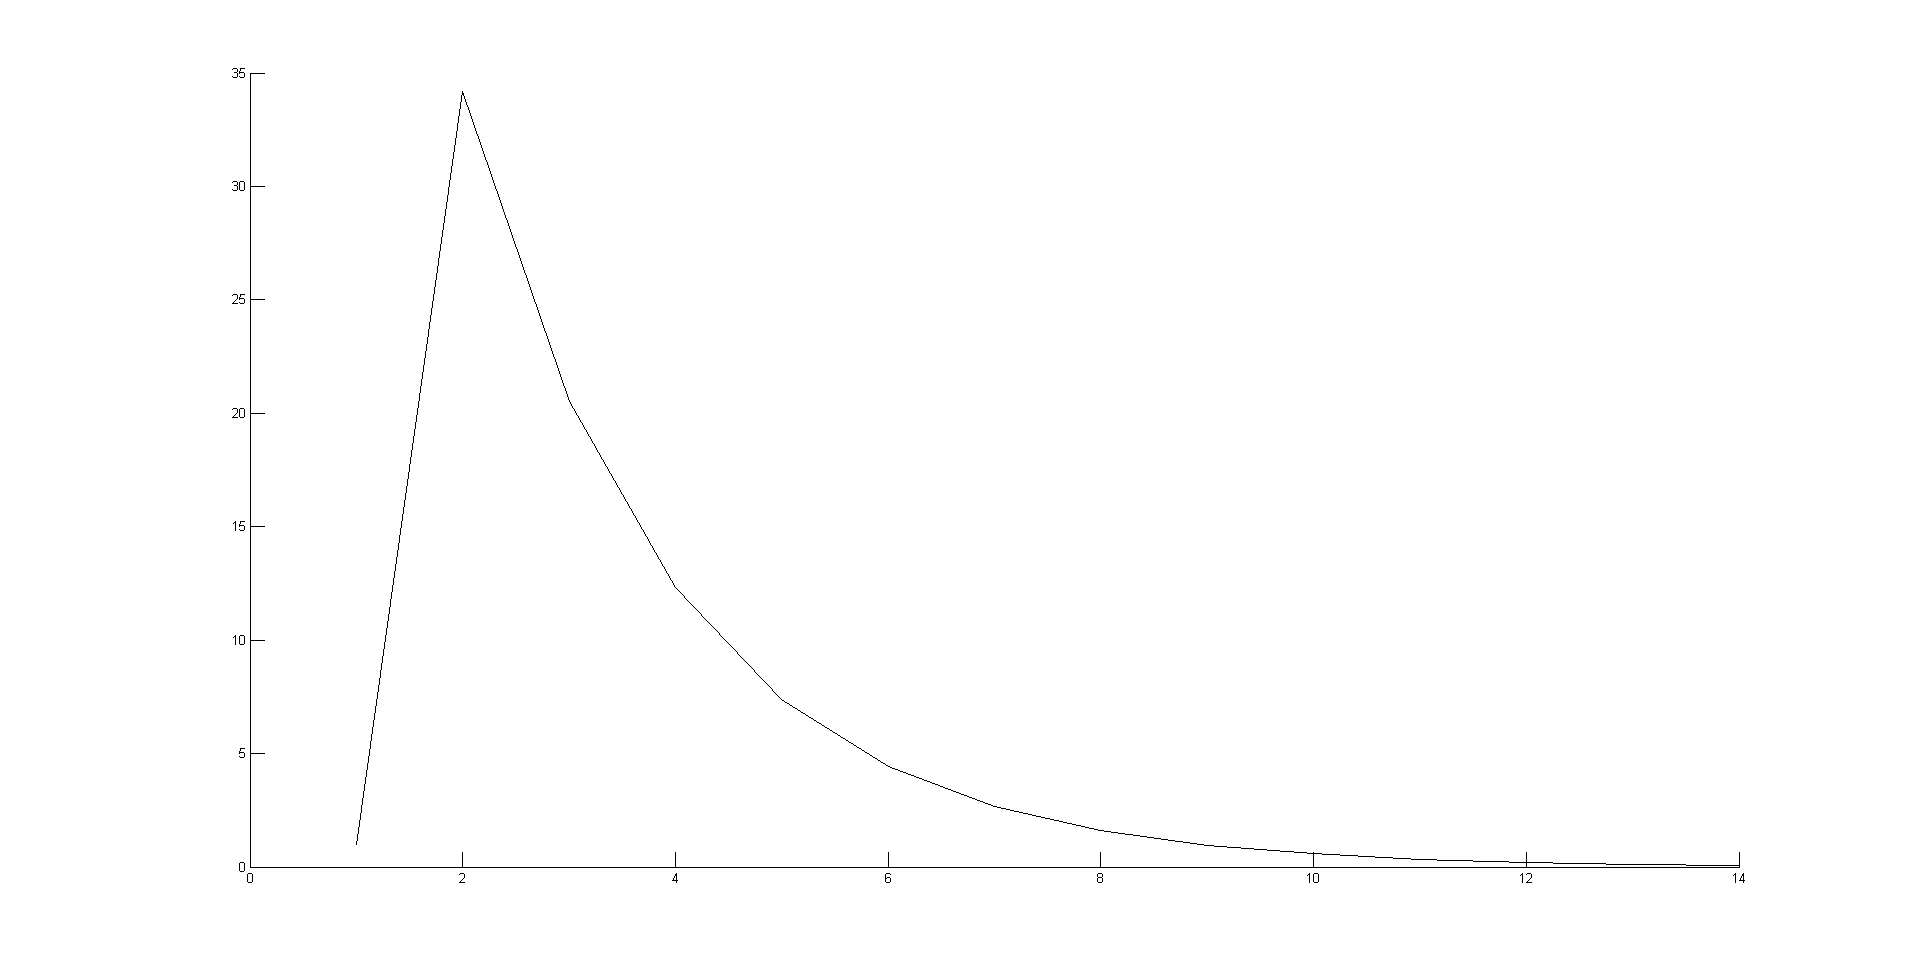
\includegraphics[width=120mm]{CW4-alg1fun1-u10_10-k01-d.png}
	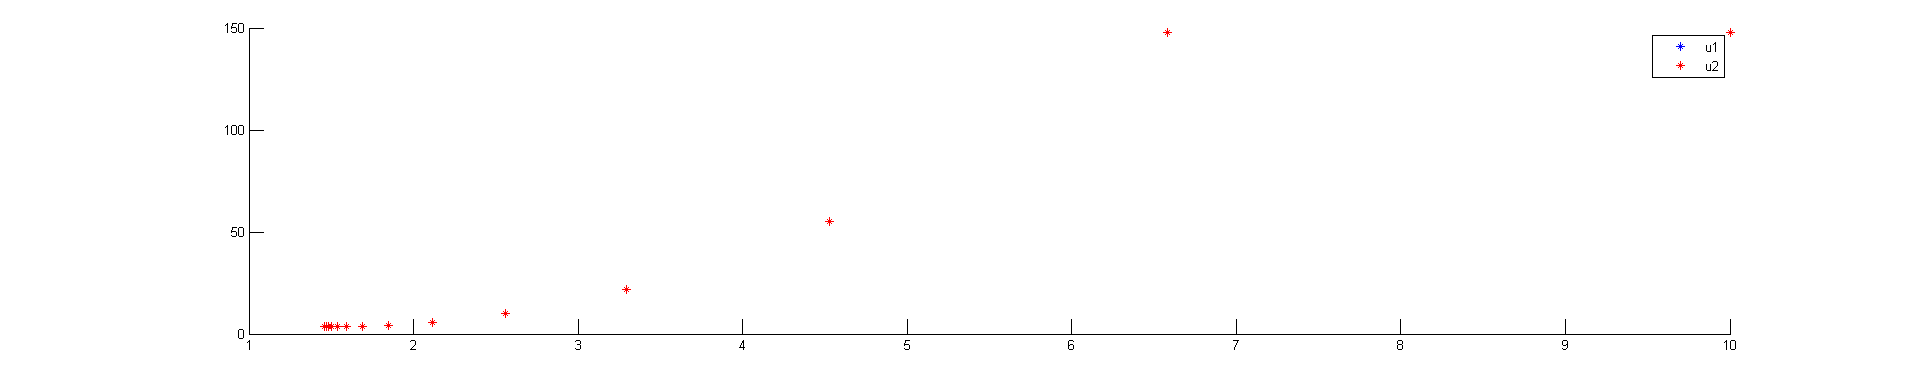
\includegraphics[width=120mm]{CW4-alg1fun1-u10_10-k01-u.png}
	\caption{Wykres wykres wartości $d$, oraz $u^{(1)}$ i $u^{(2)}$ dla $u_0=[10 \quad 10]$.}
    \label{fig:Rysunek}
\end{figure}
\begin{figure}[!h]
    \centering
	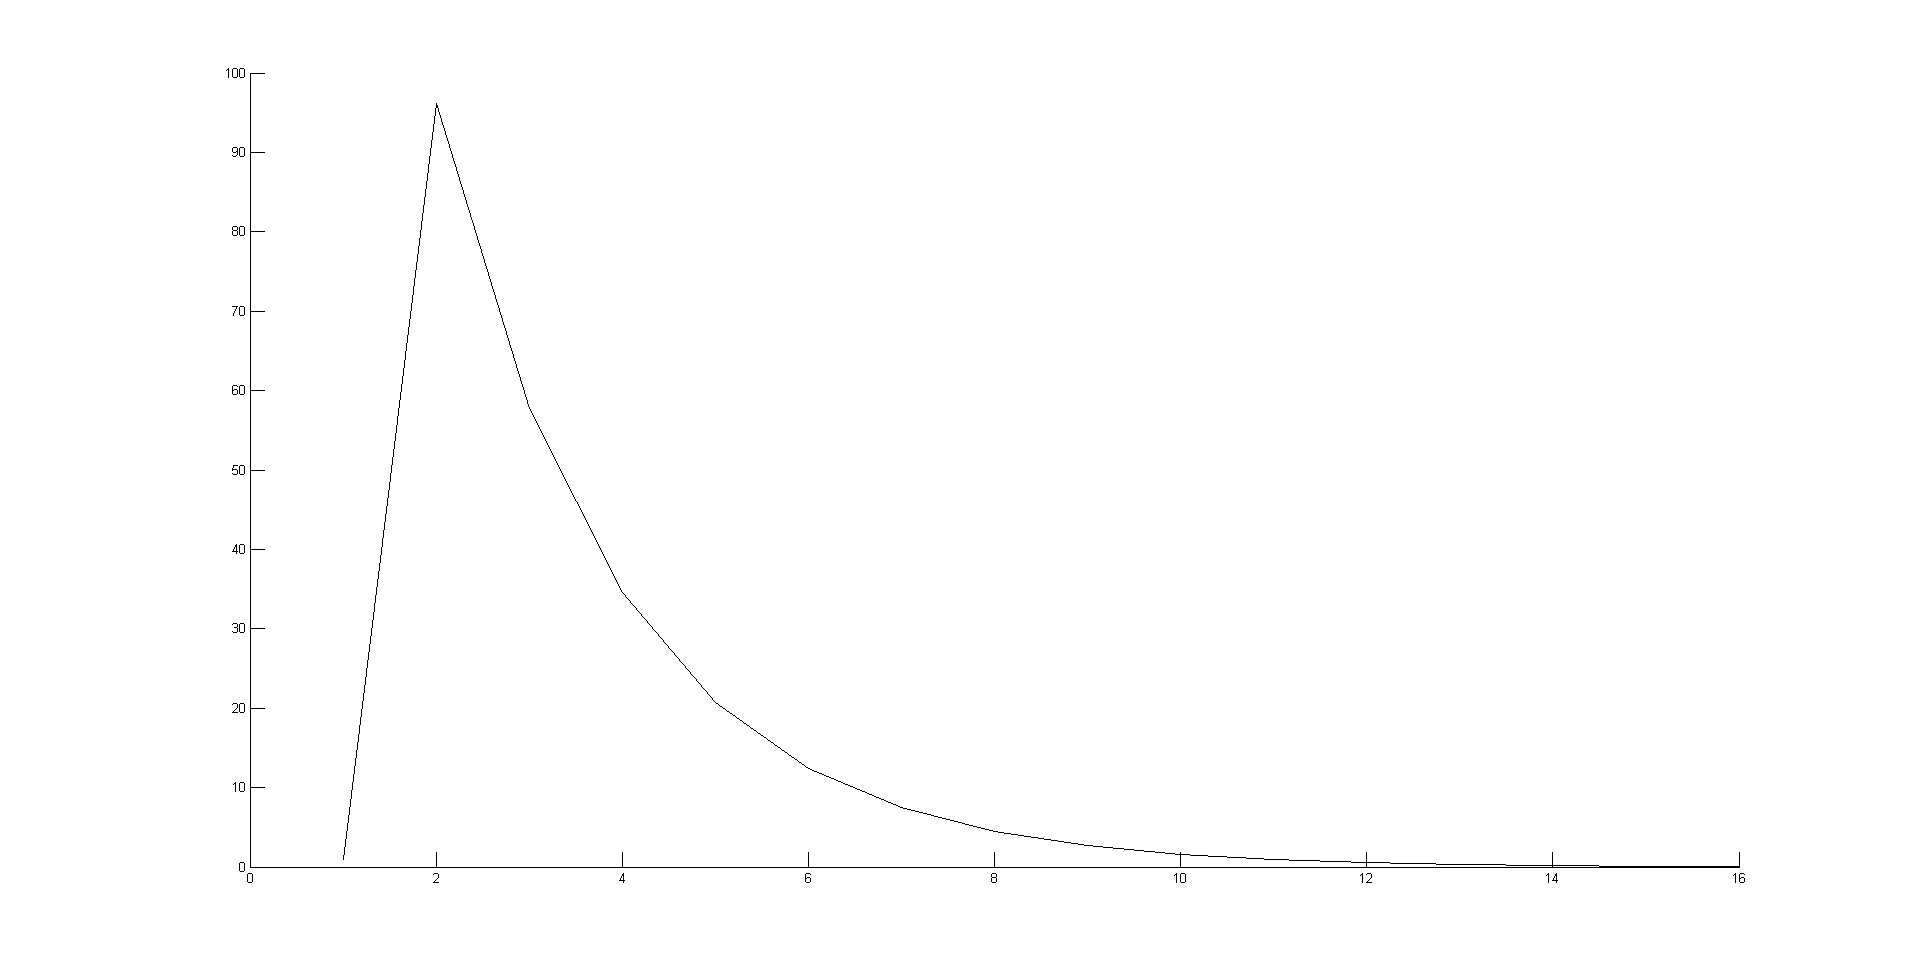
\includegraphics[width=120mm]{CW4-alg1fun1-u10_41-k01-d.png}
	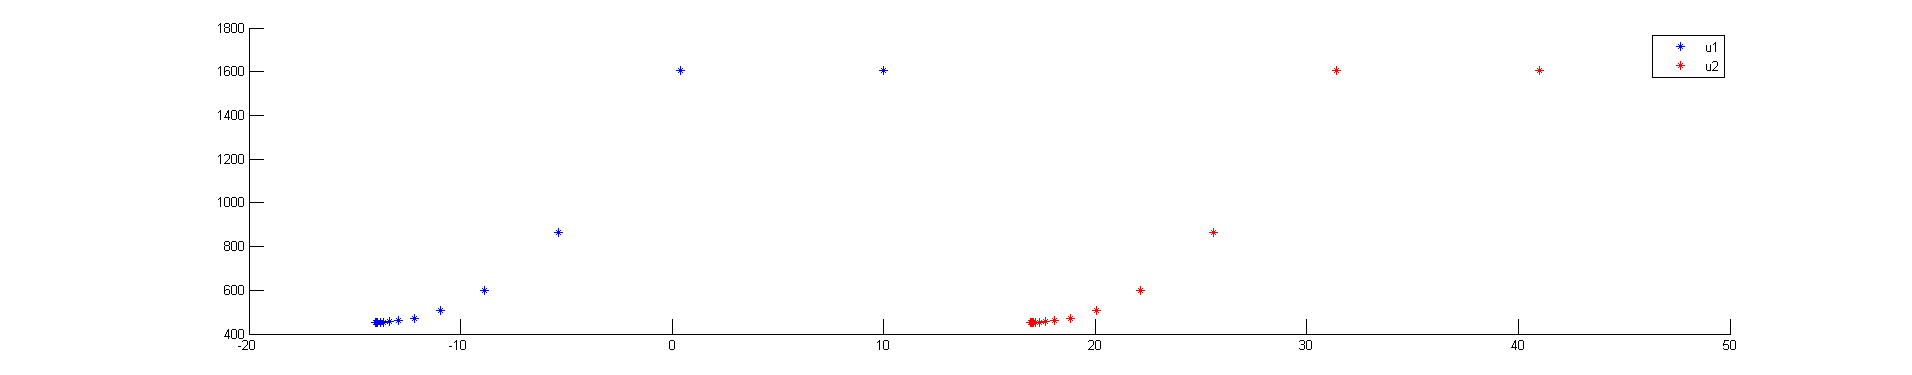
\includegraphics[width=120mm]{CW4-alg1fun1-u10_41-k01-u.png}
	\caption{Wykres wykres wartości $d$, oraz $u^{(1)}$ i $u^{(2)}$ dla $u_0=[10 \quad 41]$.}
    \label{fig:Rysunek}
\end{figure}
\begin{figure}[!h]
    \centering
	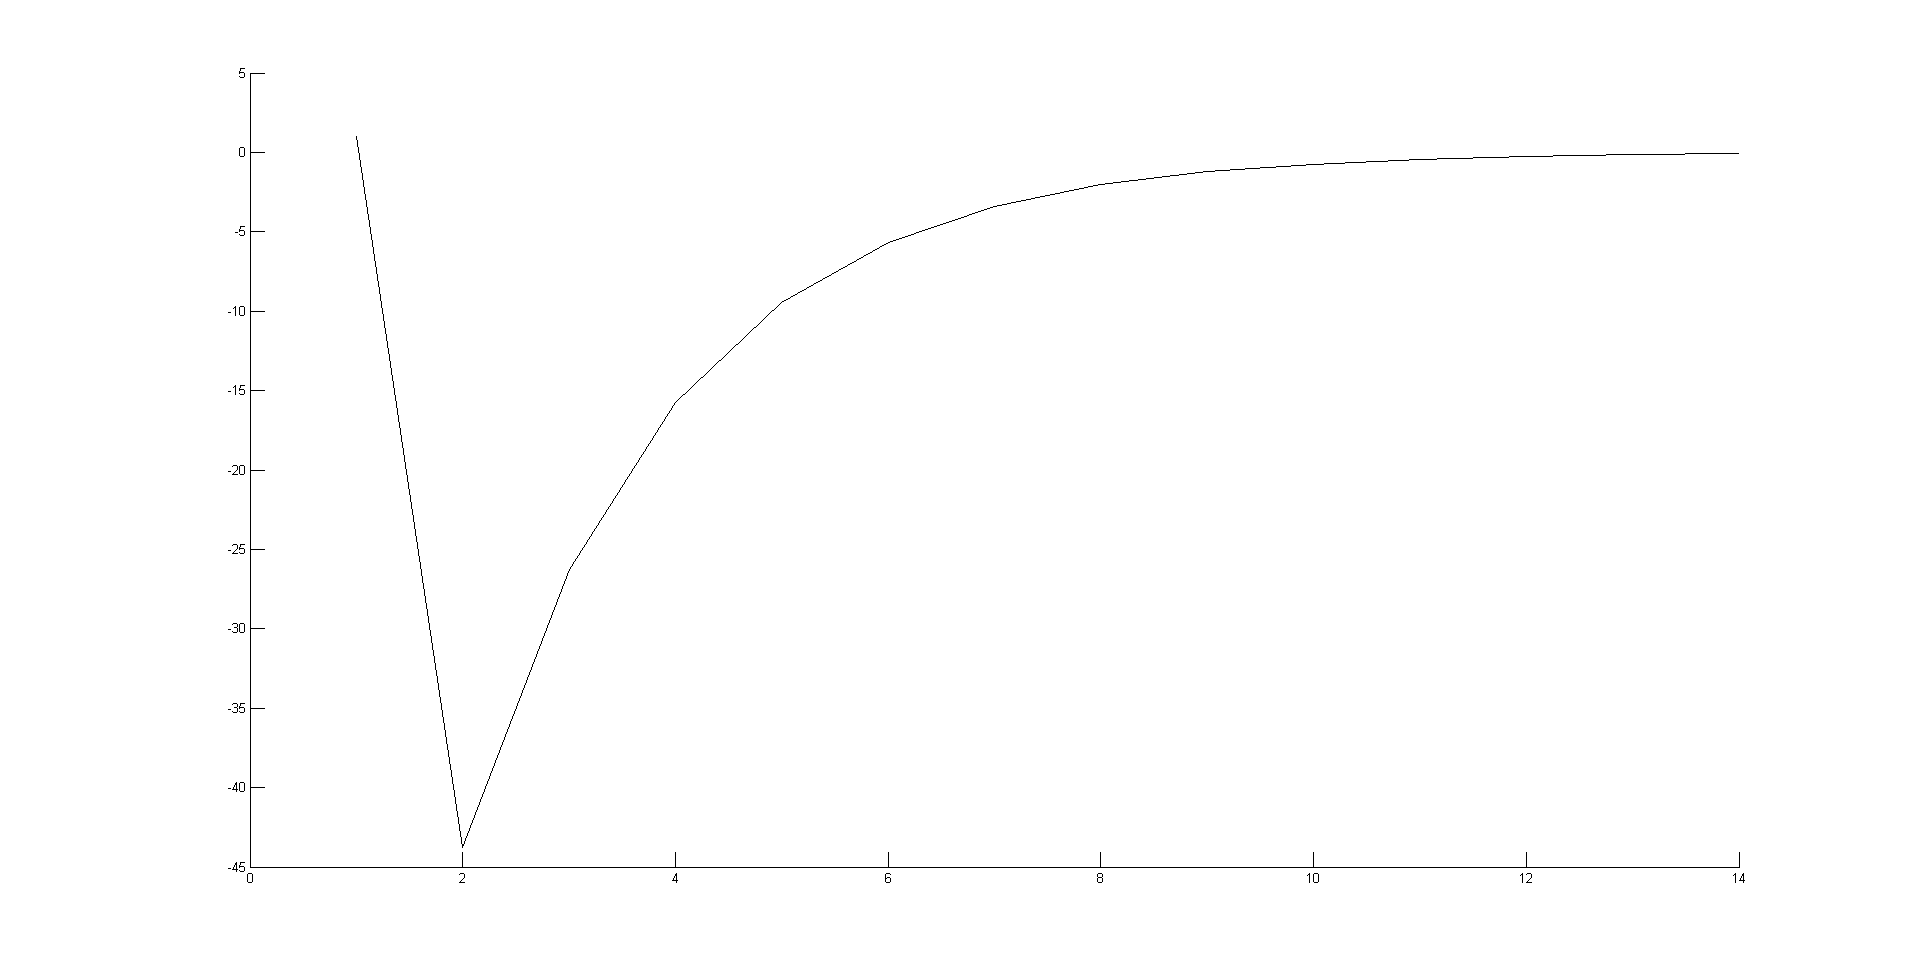
\includegraphics[width=120mm]{CW4-alg1fun1-u-24_5-k01-d.png}
	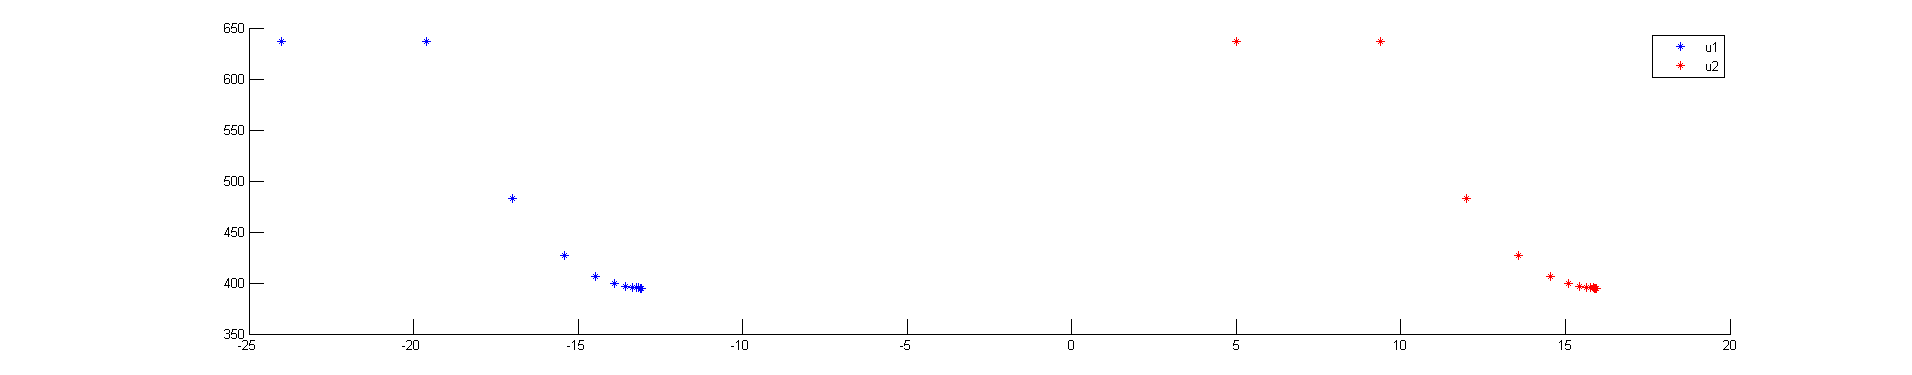
\includegraphics[width=120mm]{CW4-alg1fun1-u-24_5-k01-u.png}
	\caption{Wykres wykres wartości $d$, oraz $u^{(1)}$ i $u^{(2)}$ dla $u_0=[-24 \quad 5]$.}
    \label{fig:Rysunek}
\end{figure}

\newpage Z powyższych wykresów możemy zauważyć, że wartości $u^{(1)}$ i $u^{(2)}$ zmieniają się tak samo, a są jedynie przesunięte względem siebie o różnicę wartości początkowych $u_0^{(1)}$ i $u_0^{(2)}$, ponieważ w uproszczonym algorytmie nie mamy oddzielnych kroków $d^{(1)}$ i $d^{(2)}$ dla nich, ale jeden krok $d$ stosowany dla obu.

Następnie dla wybranych wartości początkowych wejścia $u_0$ ($[10 \quad 10]$) prześledzimy wpływ zmiany parametru $k$.

\begin{figure}[!h]
    \centering
	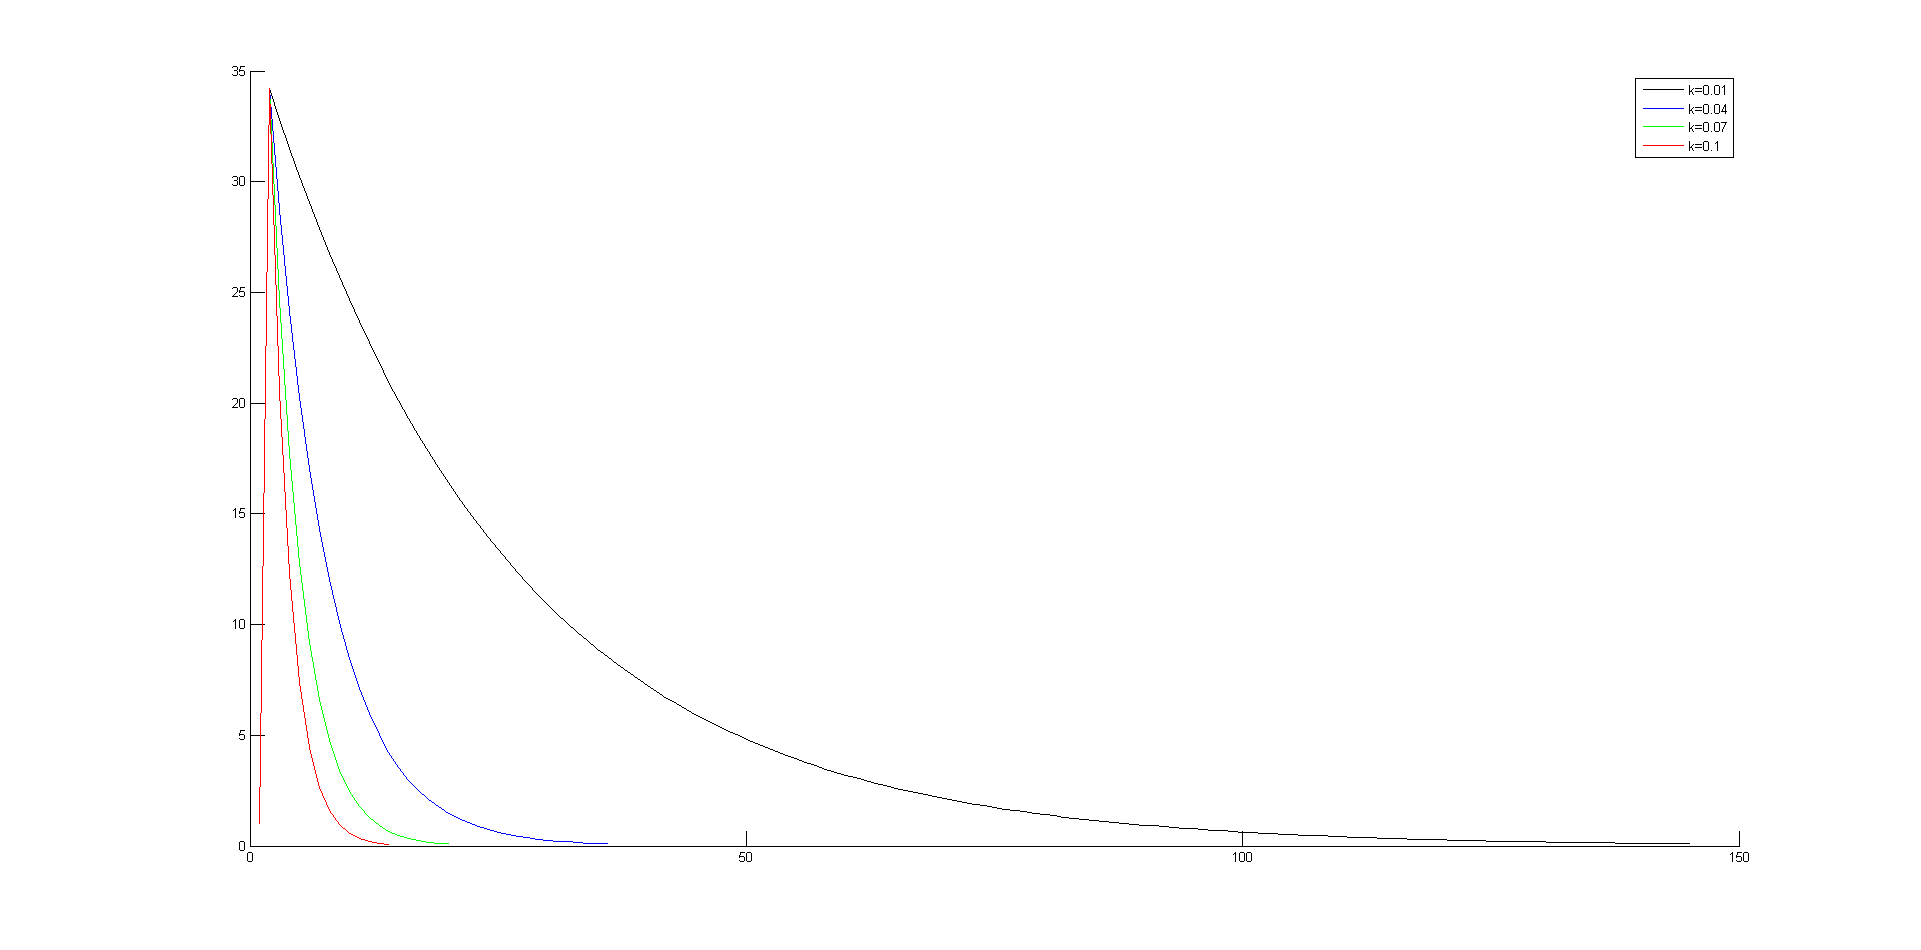
\includegraphics[width=120mm]{CW4-alg1fun1-u10_10-k001_01-d.png}
	\caption{Wykres wykres wartości $d$ przy zmianie parametru $k$.}
    \label{fig:Rysunek}
\end{figure}

Na powyższym wykresie możemy zauważyć, że w miarę zwiększania parametru $k$ wartości $d$ szybciej zbliżają się ku $0$.
\subsubsection{Obiekt (2).}
%--------------------------------------------------------------------------------------------------------------------------------
%ZADANIE 2
%--------------------------------------------------------------------------------------------------------------------------------
\subsection{Symulacja systemu sterowania ekstremalnego – wersja 1. algorytmu.}

\subsubsection{Obiekt (1).}

\subsubsection{Obiekt (2).}
%--------------------------------------------------------------------------------------------------------------------------------
%ZADANIE 3
%--------------------------------------------------------------------------------------------------------------------------------
\subsection{Symulacja systemu sterowania ekstremalnego – wersja 1. algorytmu.}

\subsubsection{Obiekt (1).}

\subsubsection{Obiekt (2).}
\section{Wnioski.}\label{sec:wnioski}

\end{document}